%%
%% File automatically generated using DocOnce (https://github.com/doconce/doconce/):
%% doconce format latex slides2.do.txt --latex_title_layout=beamer -DBEAMER --no_abort
%%
% #ifdef PTEX2TEX_EXPLANATION
%%
%% The file follows the ptex2tex extended LaTeX format, see
%% ptex2tex: https://code.google.com/p/ptex2tex/
%%
%% Run
%%      ptex2tex myfile
%% or
%%      doconce ptex2tex myfile
%%
%% to turn myfile.p.tex into an ordinary LaTeX file myfile.tex.
%% (The ptex2tex program: https://code.google.com/p/ptex2tex)
%% Many preprocess options can be added to ptex2tex or doconce ptex2tex
%%
%%      ptex2tex -DMINTED myfile
%%      doconce ptex2tex myfile envir=minted
%%
%% ptex2tex will typeset code environments according to a global or local
%% .ptex2tex.cfg configure file. doconce ptex2tex will typeset code
%% according to options on the command line (just type doconce ptex2tex to
%% see examples). If doconce ptex2tex has envir=minted, it enables the
%% minted style without needing -DMINTED.
% #endif

% #define PREAMBLE

% #ifdef PREAMBLE
%-------------------- begin preamble ----------------------

\documentclass[%
oneside,                 % oneside: electronic viewing, twoside: printing
final,                   % draft: marks overfull hboxes, figures with paths
10pt]{article}

\listfiles               %  print all files needed to compile this document

\usepackage{relsize,makeidx,color,setspace,amsmath,amsfonts,amssymb}
\usepackage[table]{xcolor}
\usepackage{bm,ltablex,microtype}

\usepackage[pdftex]{graphicx}

% Movies are handled by the href package
\newenvironment{doconce:movie}{}{}
\newcounter{doconce:movie:counter}


\usepackage{ptex2tex}
% #ifdef MINTED
\usepackage{minted}
\usemintedstyle{default}
% #endif
\usepackage{fancyvrb}

\usepackage[T1]{fontenc}
%\usepackage[latin1]{inputenc}
\usepackage{ucs}
\usepackage[utf8x]{inputenc}

\usepackage{lmodern}         % Latin Modern fonts derived from Computer Modern

% Hyperlinks in PDF:
\definecolor{linkcolor}{rgb}{0,0,0.4}
\usepackage{hyperref}
\hypersetup{
    breaklinks=true,
    colorlinks=true,
    linkcolor=linkcolor,
    urlcolor=linkcolor,
    citecolor=black,
    filecolor=black,
    %filecolor=blue,
    pdfmenubar=true,
    pdftoolbar=true,
    bookmarksdepth=3   % Uncomment (and tweak) for PDF bookmarks with more levels than the TOC
    }
%\hyperbaseurl{}   % hyperlinks are relative to this root

\setcounter{tocdepth}{2}  % levels in table of contents

% Tricks for having figures close to where they are defined:
% 1. define less restrictive rules for where to put figures
\setcounter{topnumber}{2}
\setcounter{bottomnumber}{2}
\setcounter{totalnumber}{4}
\renewcommand{\topfraction}{0.95}
\renewcommand{\bottomfraction}{0.95}
\renewcommand{\textfraction}{0}
\renewcommand{\floatpagefraction}{0.75}
% floatpagefraction must always be less than topfraction!
% 2. ensure all figures are flushed before next section
\usepackage[section]{placeins}
% 3. enable begin{figure}[H] (often leads to ugly pagebreaks)
%\usepackage{float}\restylefloat{figure}

\usepackage[framemethod=TikZ]{mdframed}

% --- begin definitions of admonition environments ---

% Admonition style "mdfbox" is an oval colored box based on mdframed
% "notice" admon
\colorlet{mdfbox_notice_background}{gray!5}
\newmdenv[
  skipabove=15pt,
  skipbelow=15pt,
  outerlinewidth=0,
  backgroundcolor=mdfbox_notice_background,
  linecolor=black,
  linewidth=2pt,       % frame thickness
  frametitlebackgroundcolor=mdfbox_notice_background,
  frametitlerule=true,
  frametitlefont=\normalfont\bfseries,
  shadow=false,        % frame shadow?
  shadowsize=11pt,
  leftmargin=0,
  rightmargin=0,
  roundcorner=5,
  needspace=0pt,
]{notice_mdfboxmdframed}

\newenvironment{notice_mdfboxadmon}[1][]{
\begin{notice_mdfboxmdframed}[frametitle=#1]
}
{
\end{notice_mdfboxmdframed}
}

% Admonition style "mdfbox" is an oval colored box based on mdframed
% "summary" admon
\colorlet{mdfbox_summary_background}{gray!5}
\newmdenv[
  skipabove=15pt,
  skipbelow=15pt,
  outerlinewidth=0,
  backgroundcolor=mdfbox_summary_background,
  linecolor=black,
  linewidth=2pt,       % frame thickness
  frametitlebackgroundcolor=mdfbox_summary_background,
  frametitlerule=true,
  frametitlefont=\normalfont\bfseries,
  shadow=false,        % frame shadow?
  shadowsize=11pt,
  leftmargin=0,
  rightmargin=0,
  roundcorner=5,
  needspace=0pt,
]{summary_mdfboxmdframed}

\newenvironment{summary_mdfboxadmon}[1][]{
\begin{summary_mdfboxmdframed}[frametitle=#1]
}
{
\end{summary_mdfboxmdframed}
}

% Admonition style "mdfbox" is an oval colored box based on mdframed
% "warning" admon
\colorlet{mdfbox_warning_background}{gray!5}
\newmdenv[
  skipabove=15pt,
  skipbelow=15pt,
  outerlinewidth=0,
  backgroundcolor=mdfbox_warning_background,
  linecolor=black,
  linewidth=2pt,       % frame thickness
  frametitlebackgroundcolor=mdfbox_warning_background,
  frametitlerule=true,
  frametitlefont=\normalfont\bfseries,
  shadow=false,        % frame shadow?
  shadowsize=11pt,
  leftmargin=0,
  rightmargin=0,
  roundcorner=5,
  needspace=0pt,
]{warning_mdfboxmdframed}

\newenvironment{warning_mdfboxadmon}[1][]{
\begin{warning_mdfboxmdframed}[frametitle=#1]
}
{
\end{warning_mdfboxmdframed}
}

% Admonition style "mdfbox" is an oval colored box based on mdframed
% "question" admon
\colorlet{mdfbox_question_background}{gray!5}
\newmdenv[
  skipabove=15pt,
  skipbelow=15pt,
  outerlinewidth=0,
  backgroundcolor=mdfbox_question_background,
  linecolor=black,
  linewidth=2pt,       % frame thickness
  frametitlebackgroundcolor=mdfbox_question_background,
  frametitlerule=true,
  frametitlefont=\normalfont\bfseries,
  shadow=false,        % frame shadow?
  shadowsize=11pt,
  leftmargin=0,
  rightmargin=0,
  roundcorner=5,
  needspace=0pt,
]{question_mdfboxmdframed}

\newenvironment{question_mdfboxadmon}[1][]{
\begin{question_mdfboxmdframed}[frametitle=#1]
}
{
\end{question_mdfboxmdframed}
}

% Admonition style "mdfbox" is an oval colored box based on mdframed
% "block" admon
\colorlet{mdfbox_block_background}{gray!5}
\newmdenv[
  skipabove=15pt,
  skipbelow=15pt,
  outerlinewidth=0,
  backgroundcolor=mdfbox_block_background,
  linecolor=black,
  linewidth=2pt,       % frame thickness
  frametitlebackgroundcolor=mdfbox_block_background,
  frametitlerule=true,
  frametitlefont=\normalfont\bfseries,
  shadow=false,        % frame shadow?
  shadowsize=11pt,
  leftmargin=0,
  rightmargin=0,
  roundcorner=5,
  needspace=0pt,
]{block_mdfboxmdframed}

\newenvironment{block_mdfboxadmon}[1][]{
\begin{block_mdfboxmdframed}[frametitle=#1]
}
{
\end{block_mdfboxmdframed}
}

% --- end of definitions of admonition environments ---

% prevent orhpans and widows
\clubpenalty = 10000
\widowpenalty = 10000

\newenvironment{doconceexercise}{}{}
\newcounter{doconceexercisecounter}


% ------ header in subexercises ------
%\newcommand{\subex}[1]{\paragraph{#1}}
%\newcommand{\subex}[1]{\par\vspace{1.7mm}\noindent{\bf #1}\ \ }
\makeatletter
% 1.5ex is the spacing above the header, 0.5em the spacing after subex title
\newcommand\subex{\@startsection{paragraph}{4}{\z@}%
                  {1.5ex\@plus1ex \@minus.2ex}%
                  {-0.5em}%
                  {\normalfont\normalsize\bfseries}}
\makeatother


% --- end of standard preamble for documents ---


% insert custom LaTeX commands...

\raggedbottom
\makeindex

%-------------------- end preamble ----------------------

\begin{document}

% matching end for #ifdef PREAMBLE
% #endif

\newcommand{\exercisesection}[1]{\subsection*{#1}}

\renewcommand{\u}{\pmb{u}}
\newcommand{\f}{\bm{f}}
\newcommand{\xbm}{\bm{x}}
\newcommand{\normalvecbm}{\bm{n}}
\newcommand{\ubm}{\bm{u}}

\newcommand{\x}{\pmb{x}}
\newcommand{\normalvec}{\pmb{n}}
\newcommand{\Ddt}[1]{\frac{D#1}{dt}}
\newcommand{\halfi}{1/2}
\newcommand{\half}{\frac{1}{2}}
\newcommand{\report}{test report}

% ------------------- main content ----------------------



% ----------------- title -------------------------

\title{Test slide features}

% ----------------- author(s) -------------------------

\author{Core Dump\inst{1}}
\institute{Cyber Space Ltd\inst{1}}
% ----------------- end author(s) -------------------------

\date{Jan 32, 2100
% <optional titlepage figure>
% <optional copyright>
}

\vspace{6mm}

% inline figure
\centerline{
\includegraphics[width=0.5\linewidth]{testfigs/doconce1b.png}}

\vspace{6mm}

% !split

% !split
\subsection{Scientific writing for the future needs to address many new media}

% !bslidecell 00 0.4

\vspace{6mm}

% inline figure
\centerline{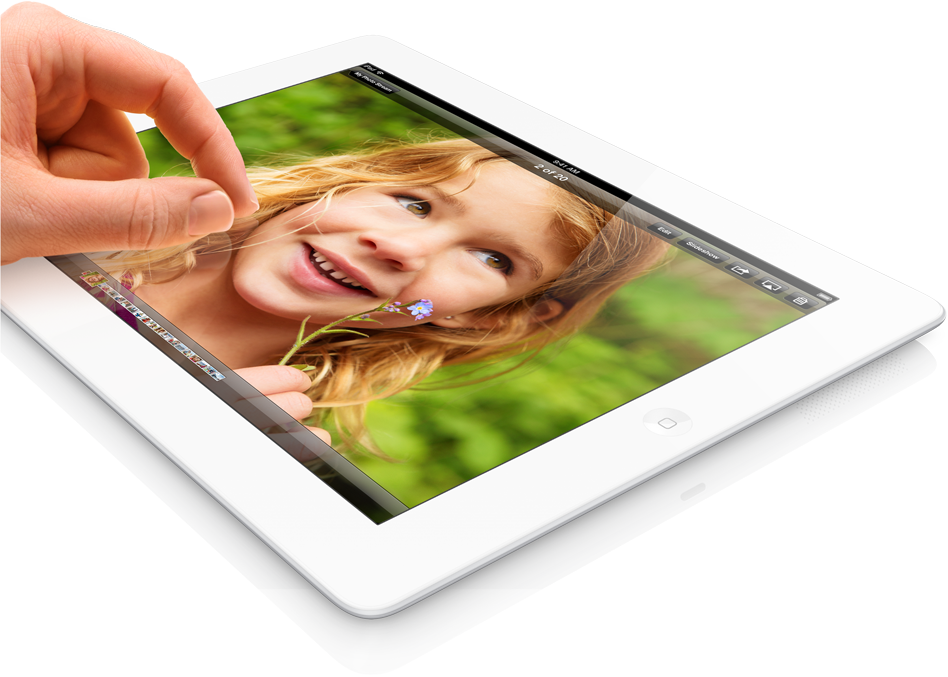
\includegraphics[width=0.8\linewidth]{testfigs/ipad.png}}

\vspace{6mm}

\vspace{6mm}

% inline figure
\centerline{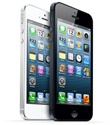
\includegraphics[width=0.3\linewidth]{testfigs/iphones.jpg}}

\vspace{6mm}

% FIGURE: [testfigs/mbair, width=400]

% !eslidecell

% !bslidecell 01 0.6

\vspace{6mm}

% inline figure
\centerline{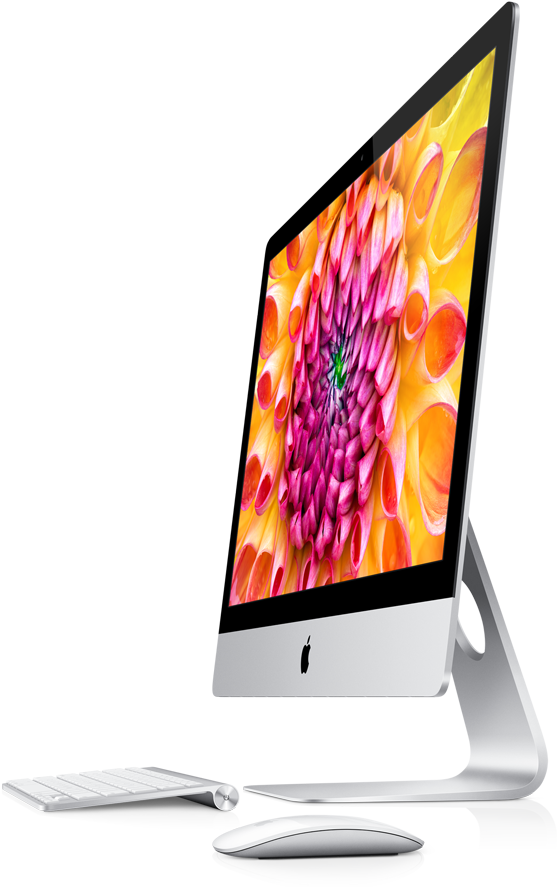
\includegraphics[width=0.7\linewidth]{testfigs/imac.png}}

\vspace{6mm}

% !eslidecell

% !split
\subsection{The book will probably survive}

\vspace{6mm}

% inline figure
\centerline{
\includegraphics[width=0.9\linewidth]{testfigs/oldbooks.jpg}}

\vspace{6mm}

% !split
\subsection{The classical report will survive}

% !bslidecell 00

\vspace{6mm}

% inline figure
\centerline{
\includegraphics[width=1.2\linewidth]{testfigs/latex_thesis.jpg}}

\vspace{6mm}

% !eslidecell

% !bslidecell 01

\vspace{6mm}

% inline figure
\centerline{
\includegraphics[width=1.2\linewidth]{testfigs/latex_paper1.png}}

\vspace{6mm}

% !eslidecell

% !split
\subsection{Scope}

% * Scientific writing = lecture notes, slides, reports, thesis, books,  ...
% * (Journal papers typeset by journals are out of scope)

% !bpop
\begin{itemize}
  \item Scope: documents with \textcolor{red}{much} \emph{math} and \emph{computer code}

  \item Key question: What tools should I use for writing?

  \item Default answer: {\LaTeX}

  \item Alternative: MS Word w/math

  \item Recent popular alternative tools: HTML w/MathJax, Sphinx, Markdown, MediaWiki, IPython notebook
\end{itemize}

\noindent
% !epop

% !bslidecell 00 0.25

\vspace{6mm}

% inline figure
\centerline{
\includegraphics[width=0.3\linewidth]{testfigs/LaTeX_logo.jpg}}

\vspace{6mm}

% !eslidecell

% !bslidecell 01 0.25

\vspace{6mm}

% inline figure
\centerline{
\includegraphics[width=0.2\linewidth]{testfigs/MS_Word_logo.jpg}}

\vspace{6mm}

% !eslidecell

% !bslidecell 02 0.5

\vspace{6mm}

% inline figure
\centerline{
\includegraphics[width=0.4\linewidth]{testfigs/sphinx_logo.png}}

\vspace{6mm}

% !eslidecell

% !bslidecell 10 0.25

\vspace{6mm}

% inline figure
\centerline{
\includegraphics[width=0.2\linewidth]{testfigs/markdown_logo.jpg}}

\vspace{6mm}

% !eslidecell

% !bslidecell 11 0.25

\vspace{6mm}

% inline figure
\centerline{
\includegraphics[width=0.2\linewidth]{testfigs/MediaWiki_logo.jpg}}

\vspace{6mm}

% !eslidecell

% !bslidecell 12 0.5

\vspace{6mm}

% inline figure
\centerline{
\includegraphics[width=0.6\linewidth]{testfigs/IPython_logo.png}}

\vspace{6mm}

% !eslidecell

% !split
\subsection{Scientific writing for the future needs to address many new media}

% Insert links here to reports

% !bslidecell 00
Old days (1985-2005): {\LaTeX} for BW paper output, but now

\begin{enumerate}
  \item BW books

  \item Colorful PDF books (printed and screen)

  \item Designed web pages

  \item Wikis

  \item Blog posts

  \item Next new fancy format (iBook w/LaTeX?)
\end{enumerate}

\noindent
% !eslidecell

% !bslidecell 01

\vspace{6mm}

% inline figure
\centerline{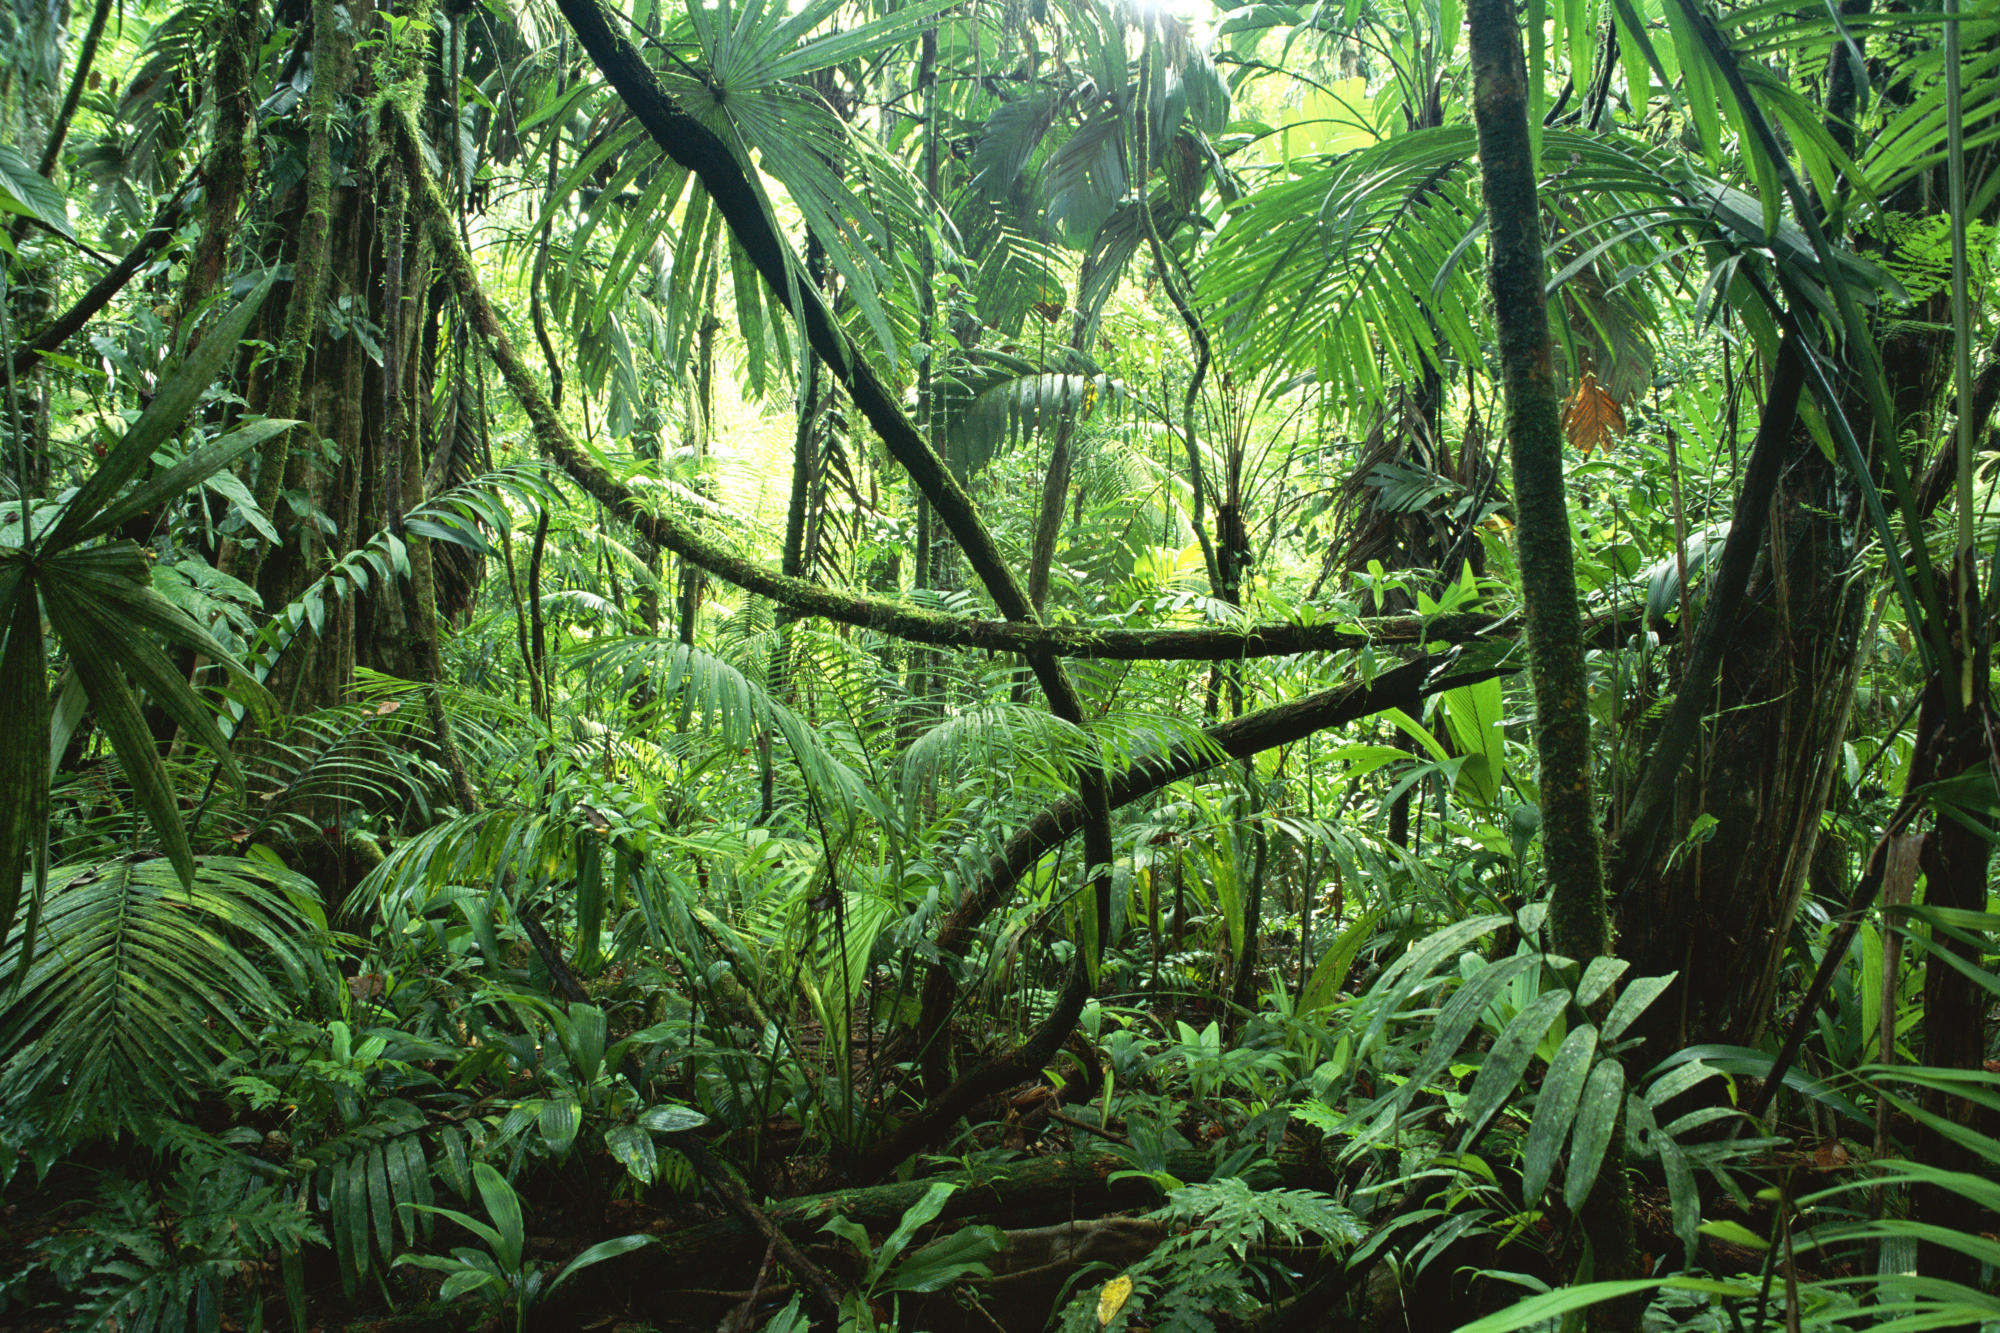
\includegraphics[width=0.9\linewidth]{testfigs/jungle_with_mess.jpg}}

\vspace{6mm}

% !eslidecell

% !split

\subsection{Fundamental question}

When I write some scientific material,

\begin{itemize}
 \item a {\LaTeX} document,

 \item a blog post (HTML),

 \item some web pages (HTML),

 \item a Sphinx document,

 \item some Markdown files,
\end{itemize}

\noindent
and later want to collect the pieces into a larger document, maybe
some book, or one big web document, is that at all feasible?

% !bpop highlight-red
Probably not, but I have a solution :-)
% !epop

% !split

\subsection{{\LaTeX} is very rich; other tools support only some elements}

\begin{itemize}
 \item {\LaTeX} inline math: works with all ({\LaTeX}, MathJax, Sphinx, Markdown, MediaWiki)

 \item {\LaTeX} equation math:
\begin{itemize}

    \item \textbf{LaTeX}: \texttt{equation*}, \texttt{equation}, \texttt{align*}, \texttt{align} + \texttt{eqnarray}, \texttt{split}, \texttt{alignat}, ... (numerous!)

    \item \textbf{MathJax}: \texttt{equation*}, \texttt{equation}, \texttt{align*}, \texttt{align}

    \item \textbf{MediaWiki}: \texttt{equation*}, \texttt{equation}, \texttt{align*}, \texttt{align}

    \item \textbf{Sphinx}: \texttt{equation*}, \texttt{equation}, \texttt{align*}

    \item \textbf{Markdown}: \texttt{equation*}, \texttt{equation}, \texttt{eqnarray*}, \texttt{align*} (but no labels)
\end{itemize}

\noindent
\end{itemize}

\noindent
% !split
\subsection{{\LaTeX} is very rich; other tools support only some elements}

% !bpop
\begin{itemize}
 \item Figures: all

 \item Subfigures: {\LaTeX} (\texttt{subfigure})

 \item Movies: {\LaTeX} (can run separately), just raw embedded HTML in others

 \item Floating computer code: {\LaTeX}

 \item Fixed computer code: all

 \item Floating tables: {\LaTeX}; inline tables: all

 \item Algorithms: {\LaTeX}

 \item Margin notes: {\LaTeX}

 \item Page references: {\LaTeX}

 \item Footnotes: {\LaTeX}, Sphinx, reStructuredText, MediaWiki

 \item Bibliography: {\LaTeX}, Sphinx, reStructuredText, MediaWiki

 \item Hyperlinks: all (but not on paper!)
\end{itemize}

\noindent
% !epop

% !bpop
Conclusion: Highly non-trivial to translate a {\LaTeX} document into something
based on HTML and vice versa.
% !epop

% !split
\subsection{DocOnce demo}

\href{{https://hplgit.github.com/teamods/writing_reports/}}{\nolinkurl{https://hplgit.github.com/teamods/writing_reports/}}

\begin{itemize}
 \item LaTeX-based PDF \href{{https://hplgit.github.com/teamods/writing_reports/_static/report.pdf}}{for screen}, \href{{https://hplgit.github.com/teamods/writing_reports/_static/report_4printing.pdf}}{for printing}, \href{{https://hplgit.github.com/teamods/writing_reports/_static/report_4phone.pdf}}{for phone}

 \item \href{{https://hplgit.github.com/teamods/writing_reports/_static/report_do.html}}{Plain HTML} or with a \href{{https://hplgit.github.com/teamods/writing_reports/_static/report_vagrant.html}}{template} or \href{{https://hplgit.github.com/teamods/writing_reports/_static/report_github_minimal.html}}{another template} or \href{{https://hplgit.github.com/teamods/writing_reports/_static/report_solarized.html}}{solarized}

 \item Sphinx: \href{{https://hplgit.github.com/teamods/writing_reports/_static/sphinx-agni/index.html}}{agni}, \href{{https://hplgit.github.com/teamods/writing_reports/_static/sphinx-pyramid/report.html}}{pyramid}, \href{{https://hplgit.github.com/teamods/writing_reports/_static/sphinx-classy/report.html}}{classy}, \href{{https://hplgit.github.com/teamods/writing_reports/_static/sphinx-fenics_minimal/report.html}}{fenics}, \href{{https://hplgit.github.com/teamods/writing_reports/_static/sphinx-fenics_minimal/report.html}}{redcloud}

 \item HTML for \href{{https://doconce-report-demo.blogspot.no/}}{Google} or \href{{https://doconcereportdemo.wordpress.com/}}{Wordpress} blog posts

 \item \href{{https://doconcedemo.shoutwiki.com/wiki/DocOnce_demo_page}}{MediaWiki} (Wikipedia, Wikibooks, etc)

 \item DocOnce \href{{https://hplgit.github.com/teamods/writing_reports/_static/report.do.txt.html}}{source code} and \href{{https://hplgit.github.io/doconce/doc/src/pub/manual/html/manual.html}}{manual}
\end{itemize}

\noindent
% !split

% latex interprets 9 = as chapter and then needs book style...
\subsection{A tour of DocOnce}

% !split
\subsection{DocOnce: title, authors, date, toc}









\bdat
TITLE: Some Title
AUTHOR: name1 at institution1, with more info & institution2
AUTHOR: name2 email:name2@web.com at institution
DATE: today

# A table of contents is optional:
TOC: on

\edat


\begin{block}{Notice}
Title and authors must have all information \emph{on a single line}!
\end{block}

% !split
\subsection{DocOnce: abstract}




\bdat
__Abstract.__
Here goes the abstract...

\edat


Or:



\bdat
__Summary.__
Here goes the summary...

\edat


% !split
\subsection{DocOnce: section headings}

Headings are surrounded by \texttt{=} signs:










\bdat
======= This is an H1/chapter heading =======

===== This is an H2/section heading =====

===== This is an H3/subsection heading =====

=== This is an H4/paragraph heading ===

__This is a paragraph heading.__

\edat


% !split
\subsection{DocOnce: markup and lists}










\bdat
 * Bullet list items start with `*`
   and may span several lines
 * *Emphasized words* are possible
 * _Boldface words_ are also possible
 * color{red}{colored words} too
 * `inline verbatim code` is featured
   o and sublists with enumerated items starting with `o`
   o items are just indented as you would do in email

\edat


This gets rendered as

\begin{itemize}
 \item Bullet lists start with \texttt{*} and may span several lines

 \item \emph{Emphasized words} are possible

 \item \textbf{Boldface words} are also possible

 \item \textcolor{red}{colored words} too

 \item \texttt{inline verbatim code} is featured
\begin{enumerate}

  \item and sublists with enumerated items starting with \texttt{o}

  \item items are just indented as you would do in email
\end{enumerate}

\noindent
\end{itemize}

\noindent
% !split
\subsection{DocOnce: labels, references, index items}






















\bdo
# Insert index items in the source
idx{key word1} idx{key word2}

# Label
===== Some section =====
label{this:section}

# Make reference
As we saw in Section ref{this:section}, references, index
items and labels follow a syntax similar to LaTeX
but without backslashes.

# Make reference to equations
See (ref{eq1})-(ref{myeq}).

# Make hyperlink
"some link text": "https://github.com/doconce/doconce"

# Hyperlink with complete URL as link text
URL: "https://github.com/doconce/doconce"

\edo


% !split
\subsection{DocOnce: figures and movies}

\begin{block}{Notice}
Figure with HTML and {\LaTeX} info, and caption, \emph{all on one line}:
\end{block}






\bdat
FIGURE: [figdir/myfig, width=300, frac=1.2] My caption. label{fig1}

# This figure will be 300 pixels wide in HTML and span 1.2 times
# the linewidth in LaTeX.

\edat


Movies are also supported:



\bdat
MOVIE: [https://www.youtube.com/embed/P8VcZzgdfSc, width=420, height=315]

\edat

and rendered as


\begin{doconce:movie}
\refstepcounter{doconce:movie:counter}
\begin{center}
\href{{https://www.youtube.com/embed/P8VcZzgdfSc}}{\nolinkurl{https://www.youtube.com/embed/P8VcZzgdfSc}}
\end{center}
\end{doconce:movie}


% !split
\subsection{DocOnce: math}

Inline math as in {\LaTeX}:



\bdat
...where $a=\int_{\Omega}fdx$ is an integral.

\edat

gets rendered as ...where $a=\int_{\Omega}fdx$ is an integral.

An equation environment is surrounded by \Verb?!bt? and \Verb?!et? tags,
the rest is plain {\LaTeX}:










\bdat
!bt
\begin{align}
\frac{\partial u}{\partial t} &= \nabla^2 u,
label{a:eq}\\
\nabla\cdot\pmb{v} & = 0
label{b:eq}
\end{align}
!et

\edat

which is rendered as

\begin{align}
\frac{\partial u}{\partial t} &= \nabla^2 u,
\label{_a:eq}\\
\nabla\cdot\pmb{v} & = 0
\label{_b:eq}
\end{align}

% !split
\subsection{DocOnce: displaying code}

Code is enclosed in \Verb?!bc? and \Verb?!ec? tags:
















\bdat
!bc pycod
def solver(I, a, T, dt, theta):
    """Solve u'=-a*u, u(0)=I, for t in (0,T] with steps of dt."""
    dt = float(dt)           # avoid integer division
    N = int(round(T/dt))     # no of time intervals
    T = N*dt                 # adjust T to fit time step dt
    u = zeros(N+1)           # array of u[n] values
    t = linspace(0, T, N+1)  # time mesh

    u[0] = I                 # assign initial condition
    for n in range(0, N):    # n=0,1,...,N-1
        u[n+1] = (1 - (1-theta)*a*dt)/(1 + theta*dt*a)*u[n]
    return u, t
!ec

\edat

This gets rendered as














\bpycod
def solver(I, a, T, dt, theta):
    """Solve u'=-a*u, u(0)=I, for t in (0,T] with steps of dt."""
    dt = float(dt)           # avoid integer division
    N = int(round(T/dt))     # no of time intervals
    T = N*dt                 # adjust T to fit time step dt
    u = zeros(N+1)           # array of u[n] values
    t = linspace(0, T, N+1)  # time mesh

    u[0] = I                 # assign initial condition
    for n in range(0, N):    # n=0,1,...,N-1
        u[n+1] = (1 - (1-theta)*a*dt)/(1 + theta*dt*a)*u[n]
    return u, t

\epycod


\begin{block}{Language-dependent typesetting of code: }
The \Verb?!bc? command can be followed by a specification of the computer
language: \texttt{pycod} for Python code snippet, \texttt{pypro} for complete Python
program, \texttt{fcod} for Fortran snippet, \texttt{fpro} for Fortran program, and so
forth (\texttt{c} for C, \texttt{cpp} for C++, \texttt{sh} for Unix shells, \texttt{m} for Matlab).
\end{block}

% !split
\subsection{DocOnce: displaying interactive demo code}
\label{slide:pot}

With \Verb?!bc pyoptpro? or a file \texttt{*.pyopt}, the code applies the
\href{{https://pythontutor.com}}{Online Python Tutor} for displaying
program flow and state of variables:
















\bpypro
def solver(I, a, T, dt, theta):
    dt = float(dt)
    N = int(round(T/dt))
    T = N*dt
    u = [0.0]*(N+1)
    t = [i*dt for i in range(N+1)]

    u[0] = I
    for n in range(0, N):
        u[n+1] = (1 - (1-theta)*a*dt)/(1 + theta*dt*a)*u[n]
    return u, t

u, t = solver(I=1, a=1, T=3, dt=1., theta=0.5)
print u

\epypro

\noindent
(\href{{https://pythontutor.com/visualize.html\#code=def+solver\%28I\%2C+a\%2C+T\%2C+dt\%2C+theta\%29\%3A\%0A++++dt+\%3D+float\%28dt\%29\%0A++++N+\%3D+int\%28round\%28T\%2Fdt\%29\%29\%0A++++T+\%3D+N\%2Adt\%0A++++u+\%3D+\%5B0.0\%5D\%2A\%28N\%2B1\%29\%0A++++t+\%3D+\%5Bi\%2Adt+for+i+in+range\%28N\%2B1\%29\%5D\%0A\%0A++++u\%5B0\%5D+\%3D+I\%0A++++for+n+in+range\%280\%2C+N\%29\%3A\%0A++++++++u\%5Bn\%2B1\%5D+\%3D+\%281+-+\%281-theta\%29\%2Aa\%2Adt\%29\%2F\%281+\%2B+theta\%2Adt\%2Aa\%29\%2Au\%5Bn\%5D\%0A++++return+u\%2C+t\%0A\%0Au\%2C+t+\%3D+solver\%28I\%3D1\%2C+a\%3D1\%2C+T\%3D3\%2C+dt\%3D1.\%2C+theta\%3D0.5\%29\%0Aprint+u&mode=display&cumulative=false&heapPrimitives=false&drawParentPointers=false&textReferences=false&py=2&curInstr=0}}{Visualize execution}) 


% !split
\subsection{DocOnce: exercises}

DocOnce offers a special format for \emph{exercises}, \emph{problems}, \emph{projects},
and \emph{examples}:

































\bdat
===== Problem: Flip a Coin =====
label{demo:ex:1}

files = flip_coin.py, flip_coin.pdf
solutions = mysol.txt, mysol_flip_coin.py
keywords = random numbers; Monte Carlo simulation

!bsubex
Make a program that simulates flipping a coin $N$ times.

!bhint
Use `r = random.random()` and define head as `r <= 0.5`.
!ehint
!esubex

!bsubex
Compute the probability of getting heads.

!bans
A short answer: 0.5.
!eans

!bsol
A full solution to this subexercise can go here.
!esol
!esubex

!bsubex
Make another program that computes the probability
of getting at least three heads out of 5 throws.
!esubex

\edat


Solutions/answers can easily be left out of the document.

% !split
\subsection{DocOnce: example on slide code}
























\bdat
!split
===== Headline =====

 * Key point 1
 * Key point 2
 * Key point 3 takes very much more text to explain because
   this point is really comprehensive, and although long
   bullet points are not recommended in general, we need
   it here for demonstration purposes

FIGURE: [testfigs/teacher1, width=100]

Key equation:

!bt
\[ -\nabla^2 u = f \quad\hbox{in }\Omega \]
!et

And maybe a final comment?

!split
===== Next slide... =====

\edat


% !split
\subsection{DocOnce: example on slide code with cells}

One can introduce a table-like layout with MxN cells and
put slide elements in various cell. A cell with position
MN is surrounded by \Verb?!bslidecell MN? and \Verb?!eslidecell?
tags. Below is an example with a bullet list to the left and
a figure to the right (two cells, numbered 00 and 01).





























\bdat
!split
===== Headline =====

!bslidecell 00
!bpop
 * Key point 1
 * Key point 2
 * Key point 3 takes very much more text to explain because
   this point is really comprehensive, and although long
   bullet points are not recommended in general, we need
   it here for demonstration purposes
!epop

!bpop
!bt
\[ -\nabla^2 u = f \quad\hbox{in }\Omega \]
!et
!epop

!eslidecell

!bslidecell 01
FIGURE: [testfigs/broken_pen_and_paper, width=400, frac=0.8]
!eslidecell

!split
===== Next slide... =====

\edat



% ------------------- end of main content ---------------

% #ifdef PREAMBLE
\cleardoublepage\phantomsection  % trick to get correct link to Index
\printindex

\end{document}
% #endif

